\chapter{Avaliações}
Esse capítulo apresenta os relatórios das avaliações realizadas.

\section{Avaliações do Protótipo de Papel}

\subsection{Relatório Consolidado - Avaliação 1 Protótipo de Papel}

\textbf{Data da avaliação:} 05/04/2015

\textbf{Objetivo:}
O objetivo dessa avaliação consistiu na elicitação de requisitos através de um teste feito em um protótipo de papel.

\textbf{Método:}
O método empregado foi o \textit{Quick and Dirty}\cite{preece}. Foi realizada em um ambiente informal e foi realizada no início do projeto.

\textbf{Usuários e perfil:}
Essa primeira avaliação foi realizada apenas com 1 usuário que se encaixava no público alvo da aplicação proposta. Foi escolhido apenas 1 usuário, pois o objetivo era obter uma rápida avaliação para elicitação de requisitos.

\textbf{Dados coletados:}
Ideias do usuário para uma tela.

\begin{table*}[!h]
\caption{Lista de problemas a ser preenchida nas avaliações. Fonte: \cite{preece} adaptado}
\label{tab:problema}
  \begin{tabular}{p{0.18\linewidth}p{0.18\linewidth}p{0.30\linewidth}p{0.30\linewidth}}
  \hline
    Nº da Iteração & ID da Questão & Questão & Recomendação\\
 \hline
    01 & 01 & Falta de uma tela intermediária entre a página inicial e a página do Matrícula Web & Construir a tela sugerida\\
  \end{tabular}
\end{table*}

\textbf{Planejamento para a próxima versão do protótipo:}
Levando em consideração os problemas encontrados será construída uma nova versão do protótipo. 
\vfill
\pagebreak

\subsection{Relatório Consolidado - Avaliação 2 Protótipo de Papel}

\textbf{Data da avaliação:} 08/05/2015

\textbf{Objetivo:}
O objetivo dessa avaliação consistiu na elicitação de requisitos através de um teste feito em um protótipo de papel.

\textbf{Método:}
O método empregado foi o \textit{Quick and Dirty} \cite{preece}. Foi realizada em um ambiente informal e foi realizada na segunda versão do protótipo construído.

\textbf{Usuários e perfil:}
Essa avaliação foi realizada com 3 usuários que se encaixavam no público alvo da aplicação proposta. Com a continuação do uso do método \textit{Quick and Dirty} os avaliadores optaram por não avaliar com muitos usuários, pois o objetivo ainda era elicitar requisitos. Assim, para não concentrar essa última avaliação do protótipo de papel em apenas um usuário, foi optado pela escolha de 3 usuários.

\textbf{Dados coletados:}
Ideias do usuário para uma tela.

\begin{table*}[!h]
\caption{Lista de problemas a ser preenchida nas avaliações. Fonte: \cite{preece} adaptado}
\label{tab:problema}
  \begin{tabular}{p{0.18\linewidth}p{0.18\linewidth}p{0.30\linewidth}p{0.30\linewidth}}
  \hline
    Nº da Iteração & ID da Questão & Questão & Recomendação\\
 \hline
    02 & 01 & Falta de uma caixa para pesquisa do nome da disciplina & Construir uma caixa de pesquisa\\
  \end{tabular}
\end{table*}

\textbf{Planejamento para a próxima versão do protótipo:}
Levando em consideração os requisitos levantados será construída uma nova versão do protótipo de papel.

\vfill
\pagebreak
\subsection{Relatório Consolidado - Avaliação 3 Protótipo de Papel}

\textbf{Data da avaliação:} 09/06/2015

\textbf{Objetivo:}
O objetivo dessa avaliação consistiu no teste da estabilidade do protótipo de papel.

\textbf{Método:}
O método empregado foi o \textit{Quick and Dirty} \cite{preece}. Foi realizada em um ambiente informal a partir da terceira versão do protótipo construído.

\textbf{Usuários e perfil:}
Essa avaliação foi realizada com 5 usuários que se encaixavam no público alvo da aplicação proposta. 
Foi consentido pelo grupo a escolha de 5 usuários, pois como objetivo era verificar a estabilidade
do protótipo foi levado em consideração o número indicado na literatura.

\textbf{Dados coletados:}

\begin{table*}[!h]
\caption{Lista de problemas. Fonte: \cite{preece} adaptado}
\label{tab:problema}
  \begin{tabular}{p{0.18\linewidth}p{0.18\linewidth}p{0.30\linewidth}p{0.30\linewidth}}
  \hline
    Nº da Iteração & ID da Questão & Questão & Recomendação\\
 \hline
    03 & 01 & Excesso de telas sem real importância & Ver necessidade da tela\\
  \end{tabular}
\end{table*}

\textbf{Planejamento para a próxima versão do protótipo:}
O protótipo será repassado para uma ferramenta.

\vfill
\pagebreak

\section{Avaliações do Protótipo da Ferramenta}

Na primeira avaliação foi pedido ao usuário que criasse uma notificação adicionando uma disciplina que aparecesse facilmente. As telas do protótipo para essa tarefa
estão na seção \ref{mobile1} no Apêndice \ref{telas_mobile}

  \subsection{Relatório Consolidado - Avaliação 1 Protótipo Ferramenta}

  \flushleft \textbf{Data da avaliação:} 
  14/06/2015

  \textbf{Objetivo:}
  Avaliar as metas e princípios da Figura \ref{Planejamento}.

  \textbf{Método:}
  O método de avaliação utilizado foi a observação direta, com a aplicação de um questionário. O questionário aplicado pode ser visto no 
  Apêndice \ref{questionário}.

  \textbf{Usuários e perfil:}
  A avaliação foi feita com 5 (cinco) usuários alvo, ou seja, utilizadores do Matrícula Web.
  
  \textbf{Dados coletados:}
   Nenhum problema foi relatado pelos usuários, por isso a tabela de problemas não foi preenchida. Os resultados coletados
   através do questionário pode ser visto na Tabela \ref{tab:resultados1}.
   
\begin{table*}[!h]
  \caption{Resultados coletados com o questionário}
  \label{tab:resultados1}
    \begin{tabular}{p{0.15\linewidth}p{0.30\linewidth}p{0.10\linewidth}p{0.10\linewidth}p{0.10\linewidth}p{0.10\linewidth}p{0.10\linewidth}}
  \hline
    ID da Questão & Meta avaliada & Resposta 1 & Resposta 2 & Resposta 3 & Resposta 4 & Resposta 5\\
  \hline
    1&Eficácia & 5 & 5 & 5 & 4 & 4\\
    2&Capacidade de aprendizado& 5 & 5 & 5 & 5 & 5 \\
    3&Utilidade& 5 & 5 & 4 &4 & 5 \\
    4&Reconhecer e diagnosticar erros& 1&1& 3& 3& 2\\
    5&Eficácia & 5 &4& 5 &4 & 5 \\
    6&Esteticamente apreciável & 5 &4 & 5 & 4 & 5\\
    7&Esteticamente apreciável & 5 & 5 & 5 & 5 &4\\
    7& Atrativo	& 5 & 5 & 5 & 5 &4\\
    8&Satisfação do usuário & 5 & 5 & 4 & 5 & 3\\
    9&Visualização do status do sistema	& 5 & 5 & 5 & 4 &1\\
    10&Reconhecer e diagnosticar erros	&1& 1& 3& 4 &2\\
    11&Visualização do status do sistema & 5 & 5 & 5 & 4&4\\

  \end{tabular}
\end{table*}

  \textbf{Sumarização dos dados coletados:}
    A partir dos dados coletados foram obtidos resultados quantitativos. Para cada meta foi calculada uma média de 1 a 5 que avalia a meta
  de muito ruim à muito bom, isso pode ser visto na Figura \ref{fig:grafico1}.
  
  \begin{figure}[h!]
  \centering
  \subfloat{
    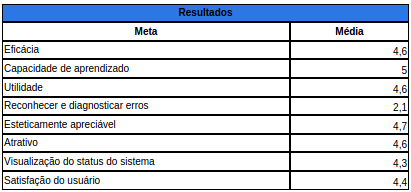
\includegraphics[keepaspectratio=true, scale=0.6]{figuras/media1.png}
   }
   \subfloat{
      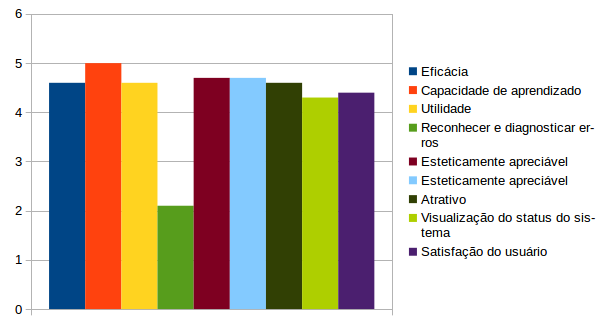
\includegraphics[keepaspectratio=true, scale=0.6]{figuras/grafico1.png}
   }
    \caption{Pontuação de cada meta avaliada na iteração}
    \label{fig:grafico1}
\end{figure}

  \textbf{Planejamento para a próxima versão do protótipo:}
  A partir dos resultados obtidos através do questionário, a próxima versão do protótipo deve possuir um maior reconhecimento e diagnosticação
  dos erros.

  \vfill
  \pagebreak

  Na segunda avaliação foi pedido ao usuário que criasse uma notificação adicionando uma disciplina que ele pesquisasse. As telas do protótipo para essa tarefa
estão na seção \ref{mobile2} no Apêndice \ref{telas_mobile}

  \subsection{Relatório Consolidado - Avaliação 2 Protótipo Ferramenta}

  \flushleft \textbf{Data da avaliação:} 
  19/06/2015

  \textbf{Objetivo:}
  Avaliar as metas e princípios da Figura \ref{Planejamento}.

  \textbf{Método:}
  O método de avaliação utilizado foi a observação direta, com a aplicação de um questionário.

  \textbf{Usuários e perfil:}
  A avaliação foi feita com 5 (cinco) usuários alvo, ou seja, utilizadores do Matrícula Web.

  \textbf{Dados coletados:}
     Nenhum problema foi relatado pelos usuários, por isso a tabela de problemas não foi preenchida. Os resultados coletados
   através do questionário pode ser visto na Tabela \ref{tab:resultados2}.
   
\begin{table*}[!h]
  \caption{Resultados coletados com o questionário}
  \label{tab:resultados2}
    \begin{tabular}{p{0.15\linewidth}p{0.30\linewidth}p{0.10\linewidth}p{0.10\linewidth}p{0.10\linewidth}p{0.10\linewidth}p{0.10\linewidth}}
  \hline
    ID da Questão & Meta avaliada & Resposta 1 & Resposta 2 & Resposta 3 & Resposta 4 & Resposta 5\\
  \hline
    1&Eficácia &5&5&4&5&5\\
     2&Capacidade de aprendizado &5&4&5&4&5\\
      3&Utilidade&5&4&5&2&5\\
      4&Reconhecer e diagnosticar erros&3&3&3&3&4\\
      5&Ajuda e documentação&5&5&5&4&5\\
      6&Estética e design minimalista&5&5&5&5&5\\
      7&Esteticamente apreciável&5&4&4&5&5\\
      7&Atrativo&5&4&4&5&5\\
       8&Esteticamente apreciável &5&4&5&4&5\\
        8&Atrativo&5&4&5&4&5\\
     9&Visualização do status do sistema &5&4&4&5&5\\
      10&Reconhecer e diagnosticar erros &3&3&3&3&4\\
      11&Visualização do status do sistema &5&5&5&3&5\\
      12&Eficiência e Eficácia &3&5&4&4&5\\
      13&Ajuda e documentação&5&3&5&3&4\\
      14&Eficiência&5&5&4&5&5\\
      15&Estética e design minimalista&4&5&5&5&5\\
      16&Satisfação do usuário&5&5&4&3&5\\
      17&Controle e liberdade do usuário&4&5&5&5&5\\
      18&Capacidade de aprendizado&3&5&3&5&5\\
      19&Utilidade&5&4&5&5&5\\

  \end{tabular}
\end{table*}

  \textbf{Sumarização dos dados coletados:}
  A partir dos dados coletados foram obtidos resultados quantitativos. Para cada meta foi calculada uma média de 1 a 5 que avalia a meta
  de muito ruim à muito bom, isso pode ser visto na Figura \ref{fig:grafico2}.
  \pagebreak
  \begin{figure}[h!]
  \centering
  \subfloat{
    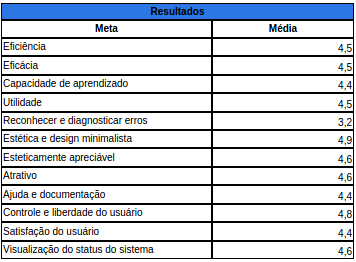
\includegraphics[keepaspectratio=true, scale=0.6]{figuras/media2.png}
   }
   \subfloat{
      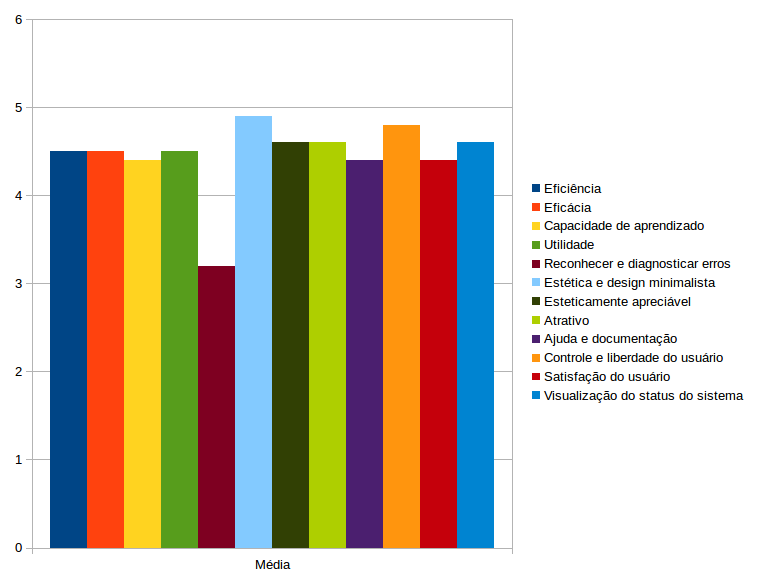
\includegraphics[keepaspectratio=true, scale=0.6]{figuras/grafico2.png}
   }
    \caption{Pontuação de cada meta avaliada na iteração}
    \label{fig:grafico2}
\end{figure}
  
  Para essa avaliação as métricas propostas no Planejamento foram coletadas e os seus resultados podem ser vistos na Figura \ref{fig:metricas}.
  
  \begin{figure}[h!]
  \centering
    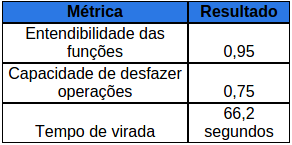
\includegraphics[keepaspectratio=true, scale=0.6]{figuras/metricas.png}
  \caption{Resultado das métricas de qualidade coletadas}
  \label{fig:metricas}
\end{figure}

  \textbf{Planejamento para a próxima versão do protótipo:}
  A partir dos resultados obtidos através do questionário e das métricas de qualidade, conclui-se que o protótipo atende as metas
  e princípios predeterminados. Porém, as notas para o princípio de usabilidade: Reconhecer e diagnosticar erros; indicam que as atividades
  propostas para a avaliação não foram suficientes para a completa análise desse princípio, o que explica sua nota mediana. Contudo, os
  resultados obtidos foram satisfatórios, portanto, não há necessidade de uma nova versão do protótipo.

  \vfill
  \pagebreak
\section{Avaliação de Acessibilidade}
Um protótipo \textit{desktop} foi realizado para avaliar a acessibilidade da aplicação e o contraste de cores. As telas avaliadas
podem ser vistas no Apêndice \ref{telas_desktop}.
\subsection{Relatório Consolidado - Avaliação 1 Acessibilidade}

\flushleft \textbf{Data da avaliação:} 
06/06/2015

\textbf{Objetivo:}
Avaliar a acessibilidade da aplicação, ou seja, o quanto ela está adequada para pessoas portadoras de algum tipo
de necessidade especial.

\textbf{Método:}
Ferramenta ASES.

\textbf{Dados coletados:}
Para construção desse protótipo foram levadas em consideração as características contidas na Tabela \ref{tab:emag} e 
as considerações provenientes do \cite{emag}. Assim, este protótipo foi construído de forma a obter um resultado
satisfatório no quesito acessibilidade.

Os dados coletados na ferramenta ASES podem ser vistos na Figura \ref{fig:avaliacao_ases1}.

\begin{figure}[h!]
  \centering
    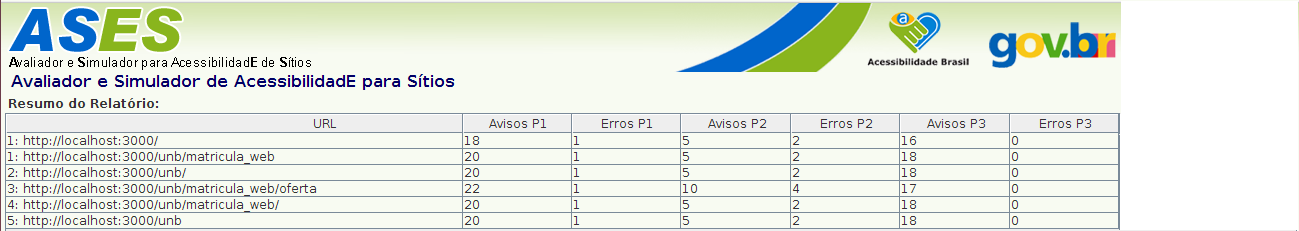
\includegraphics[keepaspectratio=true, scale=0.6]{figuras/avaliacao_ases1.png}
  \caption{Resultado da primeira avaliação da ferramenta ASES}
  \label{fig:avaliacao_ases1}
\end{figure}

Também foi avaliado o contraste de cor entre alguns objetos da tela. Os dados da avaliação contraste podem ser vistos nas Figuras \ref{fig:contraste1} e \ref{fig:contraste1b}.

Na Figura \ref{fig:contraste1}a está representado o contraste entre o fundo do menu e os links e na \ref{fig:contraste1}b entre a cor do botão e o nome de pesquisa.
\begin{figure}[h!]
  \centering
  \subfloat[a]{
    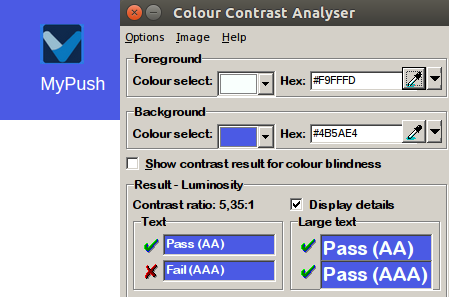
\includegraphics[keepaspectratio=true, scale=0.6]{figuras/contraste1.png}
   }
   \subfloat[b]{
      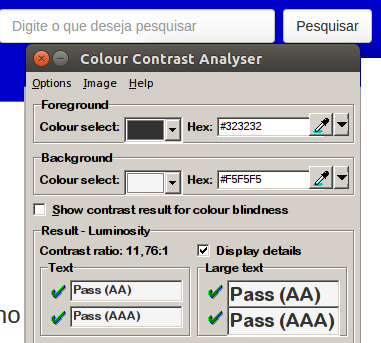
\includegraphics[keepaspectratio=true, scale=0.6]{figuras/contraste_pesquisa.png}
   }
    \caption{Resultado da avaliação de contraste}
    \label{fig:contraste1}
\end{figure}

Na Figura \ref{fig:contraste1b}a está representado o contraste entre o fundo da página e o texto escrito e na \ref{fig:contraste1b}b entre o fundo da página e a seta.
\begin{figure}[h!]
  \centering
  \subfloat[a]{
    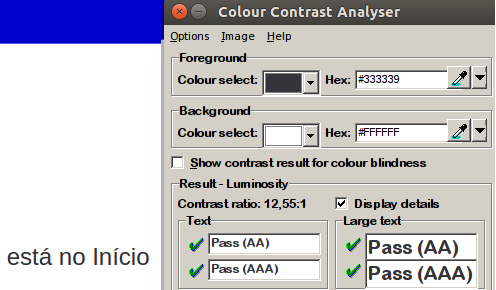
\includegraphics[keepaspectratio=true, scale=0.5]{figuras/contraste_palavra.png}
   }
   \subfloat[b]{
      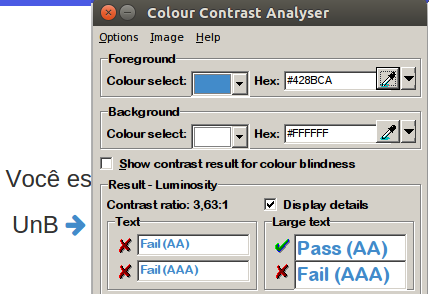
\includegraphics[keepaspectratio=true, scale=0.5]{figuras/contraste_seta1.png}
    }
    \caption{Resultado da avaliação de contraste}
    \label{fig:contraste1b}
\end{figure}

\textbf{Planejamento para a próxima versão do protótipo:}
A partir dos dados coletados serão feitos os ajustes recomendados pela ferramenta ASES e serão procuradas cores que passem em todas
as categorias da avaliação de contraste.

\vfill
\pagebreak


\subsection{Relatório Consolidado - Avaliação 2 Acessibilidade}

\flushleft \textbf{Data da avaliação:} 
20/06/2015

\textbf{Objetivo:}
Avaliar a acessibilidade da aplicação, ou seja, o quanto ela está adequada para pessoas portadoras de algum tipo
de necessidade especial.

\textbf{Método:}
Ferramenta ASES e \textit{Colour Contrast Analyser}.

\textbf{Dados coletados:}
Após as melhorias feitas com base na primeira avaliação, os dados coletados na ferramenta ASES podem ser vistos na Figura \ref{fig:avaliacao_ases}.

\begin{figure}[h!]
  \flushleft
    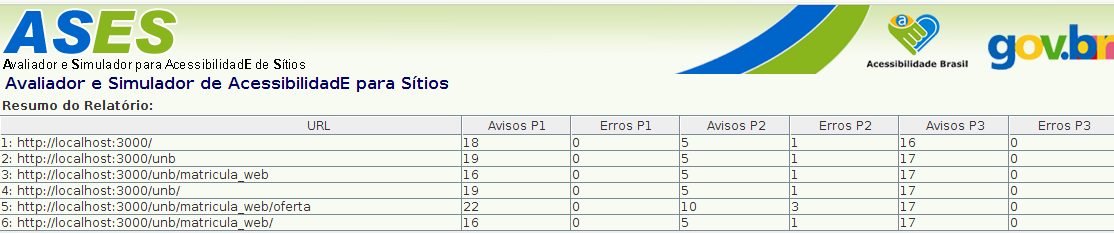
\includegraphics[keepaspectratio=true, scale=0.6]{figuras/avaliacao_ases.png}
  \caption{Resultado da segunda avaliação da ferramenta ASES}
  \label{fig:avaliacao_ases}
\end{figure}

Com essa avaliação é notório que a aplicação tem poucos erros em relação à acessibilidade e possui alguns avisos.
A partir desses avisos foi possível ajustar o código de modo a deixar a aplicação mais acessível, contudo a ferramenta não
identificou esses ajustes. Assim, o erro que persistiu após a avaliação foi ajustado no código, mas não foi reconhecido pela ferramenta.

Também foi avaliado o contraste de cor entre os objetos que mudaram de cor desde a última avaliação. As avaliações podem ser vistas nas Figuras 
\ref{fig:contraste2}. Na Figura \ref{fig:contraste2}a está representado o contraste entre o fundo do menu e os links e na \ref{fig:contraste2}b entre o fundo da página e a seta.

\begin{figure}[h!]
  \centering
  \subfloat[a]{
    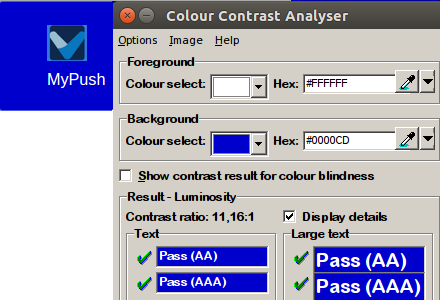
\includegraphics[keepaspectratio=true, scale=0.5]{figuras/contraste2.png}
   }
   \subfloat[b]{
      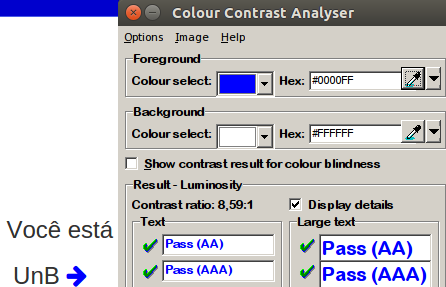
\includegraphics[keepaspectratio=true, scale=0.5]{figuras/contraste_seta2.png}
   }
    \caption{Resultado da avaliação de contraste}
    \label{fig:contraste2}
\end{figure}



\textbf{Planejamento para a próxima versão do protótipo:}
Como os ajustes foram feitos mas não identificados pela ferramenta, o protótipo foi considerado estável para o seu fim.

\vfill
\pagebreak




